% 图 77.4 —— 由 `checks/emit_hand.py` 自动拼出（probe 精测 + prims2 图元分解）
%%
% ⚠ 这是**稿子不是成品**：跑 `checks/checkhand.py 77.4` 看指标 + 看叠合图。
%%
%% ⚠ 待核：
%   · 本图 probe 报出阴影族 2 个 —— **本脚本不生成阴影**（要照原书手写）；prims2 的 strokes 里可能含阴影线，核对时留意别画重
%   · 可疑字形 1 项（空心圈 ⊙ 常被认成字母 o）—— 见文件末
%%
\documentclass[12pt]{standalone}
\usepackage{fontspec}
\setsansfont{Arial}
\newfontfamily\mfallback{DejaVu Sans}
\usepackage{tikz}
\begin{document}
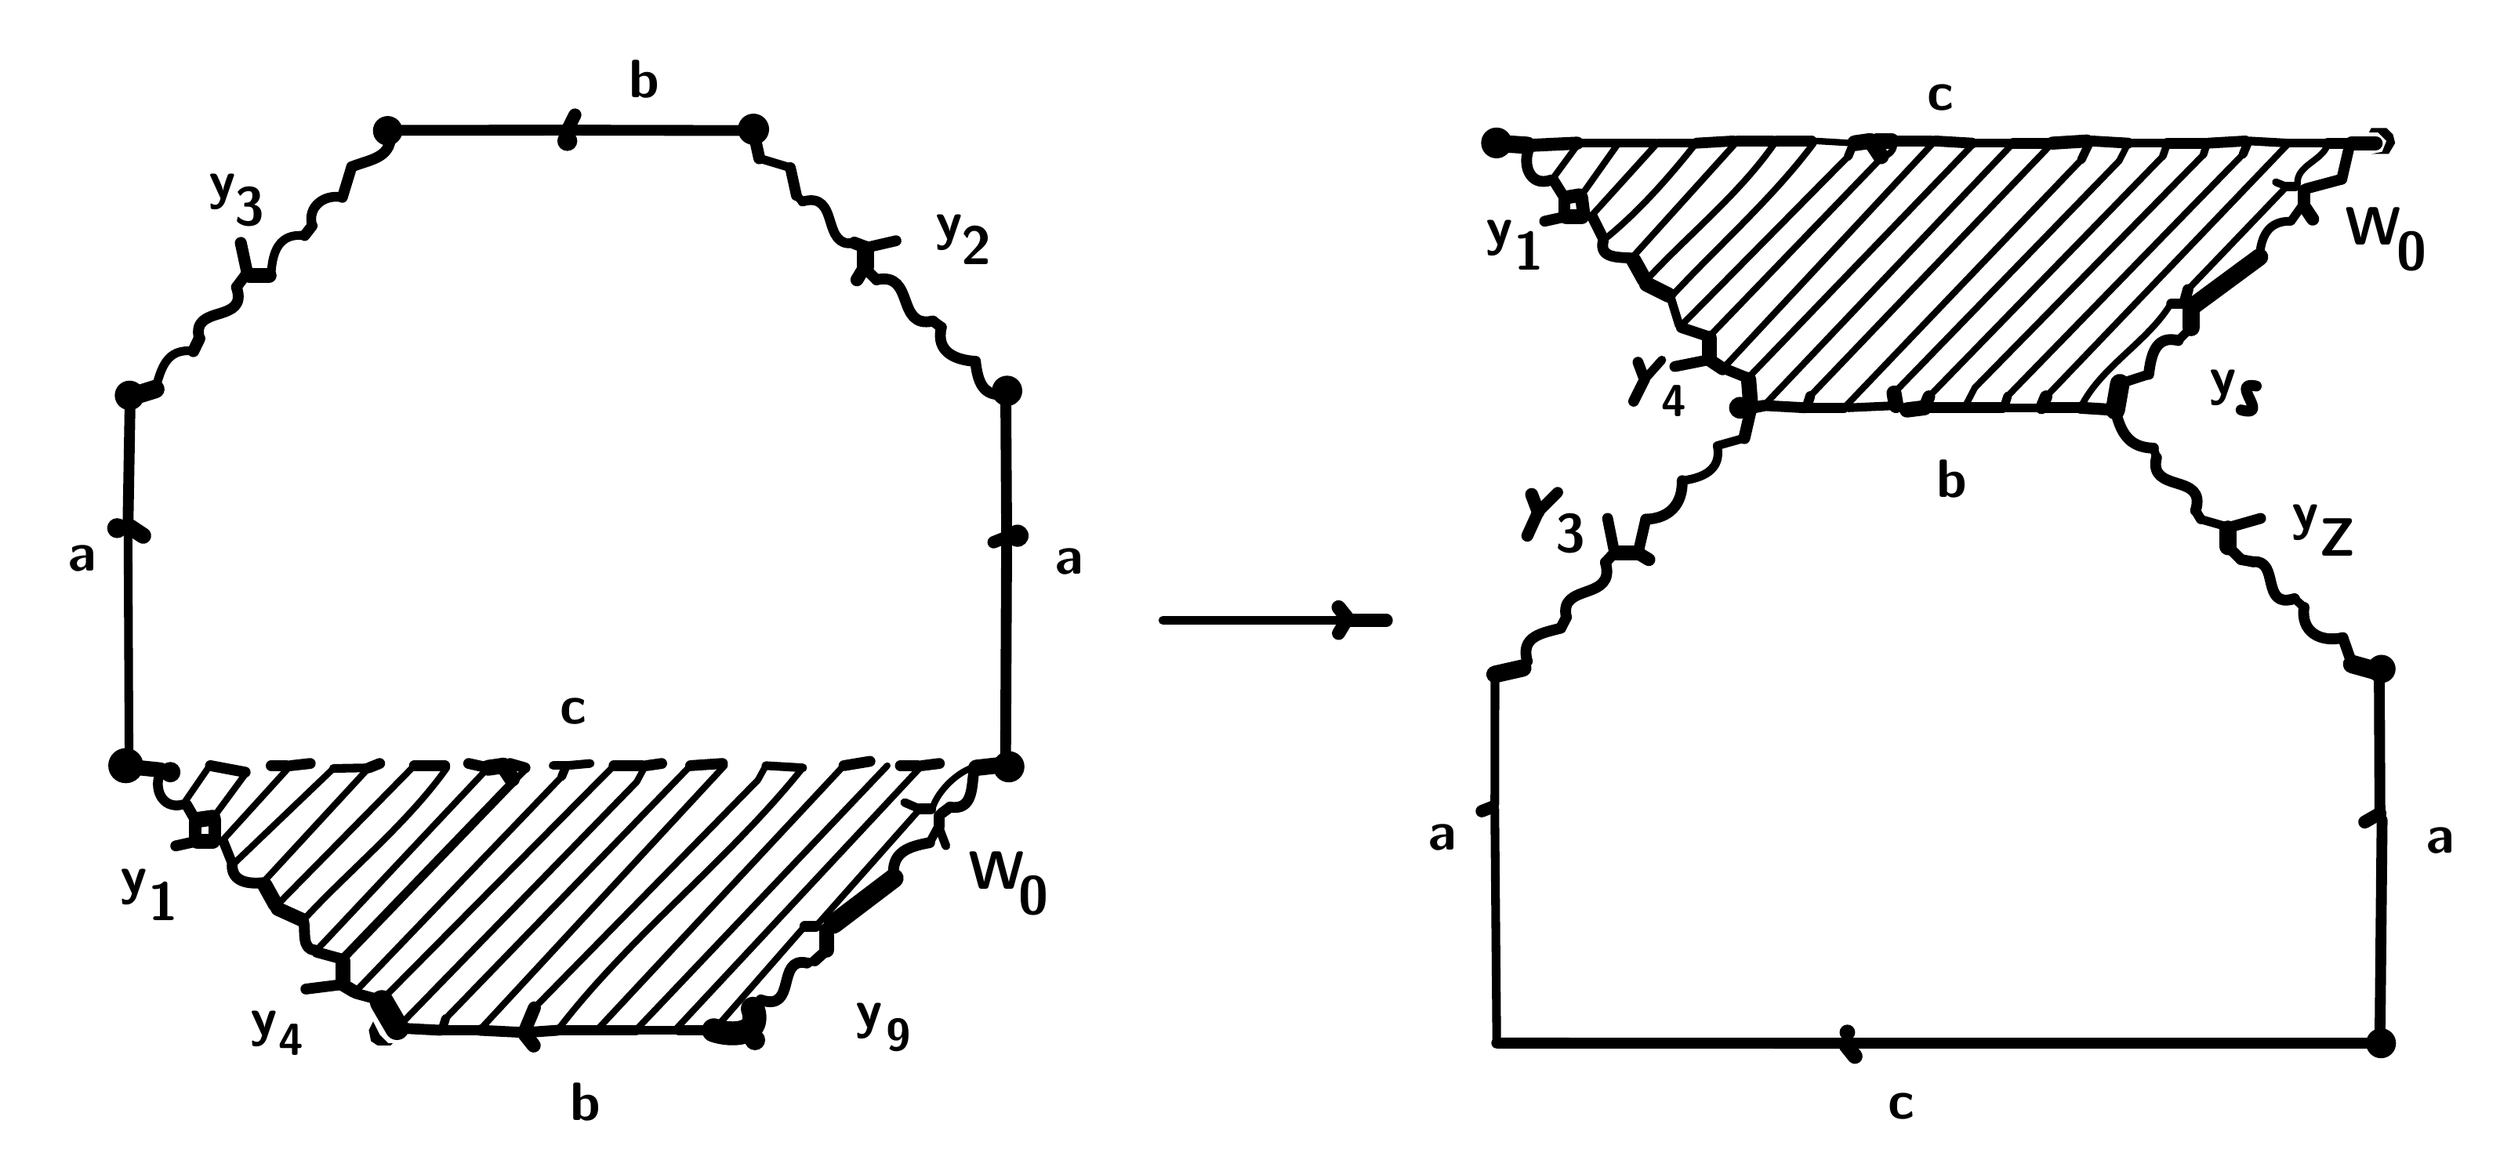
\begin{tikzpicture}[x=1pt, y=-1pt, line width=3.0pt, line cap=round, line join=round]

  %% ════ 填充区（prims2 的 fills）════
  \fill (1083.0,49.0) -- (1082.0,51.0) -- (1086.0,51.0) -- (1090.0,55.0) -- (1088.0,60.0) -- (1083.0,61.0) -- (1091.0,61.0) -- (1094.0,56.0) -- (1093.0,52.0) -- (1090.0,49.0) -- cycle;
  \fill (162.0,461.0) -- (160.0,465.0) -- (161.0,470.0) -- (164.0,472.0) -- (170.0,472.0) -- (171.0,471.0) -- (169.0,471.0) -- (165.0,467.0) -- cycle;

  %% ════ 直线段（prims2 的 strokes）════
  \draw[line width=3.0pt] (724.0,89.0) -- (753.0,57.0);
  \draw[line width=5.7pt] (453.0,238.0) -- (448.0,240.0);
  \draw[line width=5.0pt] (253.0,50.0) -- (337.2,50.2);
  \draw[line width=5.5pt] (337.2,50.2) -- (340.0,63.0);
  \draw[line width=4.0pt] (340.0,63.0) -- (354.3,67.3);
  \draw[line width=5.0pt] (354.3,67.3) -- (357.1,80.1);
  \draw[line width=4.0pt] (357.1,80.1) -- (359.9,82.9);
  \draw[line width=5.8pt] (383.8,102.0) -- (389.0,104.0);
  \draw[line width=5.0pt] (731.0,229.0) -- (734.0,244.0);
  \draw[line width=3.0pt] (154.0,447.0) -- (248.9,348.1);
  \draw[line width=4.0pt] (248.9,348.1) -- (251.0,343.0);
  \draw[line width=7.3pt] (852.0,55.0) -- (845.0,56.0);
  \draw[line width=6.0pt] (148.0,444.0) -- (153.0,447.0);
  \draw[line width=7.0pt] (117.0,407.0) -- (112.0,398.0);
  \draw[line width=4.5pt] (823.0,177.0) -- (824.4,172.6);
  \draw[line width=3.0pt] (824.4,172.6) -- (935.0,57.0);
  \draw[line width=7.0pt] (759.0,126.0) -- (749.0,121.0);
  \draw[line width=7.0pt] (797.0,178.0) -- (796.0,165.0);
  \draw[line width=5.0pt] (154.0,448.0) -- (165.0,451.0);
  \draw[line width=6.1pt] (607.0,282.0) -- (610.0,277.0);
  \draw[line width=3.0pt] (841.0,177.0) -- (949.4,63.6);
  \draw[line width=4.0pt] (949.4,63.6) -- (953.0,56.0);
  \draw[line width=7.0pt] (869.0,179.0) -- (877.0,178.0);
  \draw[line width=7.4pt] (56.0,237.0) -- (50.0,233.0);
  \draw[line width=5.0pt] (734.0,245.0) -- (730.0,249.3);
  \draw[line width=5.0pt] (712.0,274.6) -- (709.4,279.6);
  \draw[line width=3.8pt] (694.0,294.9) -- (691.9,298.0);
  \draw[line width=8.0pt] (691.9,298.0) -- (679.1,300.9);
  \draw[line width=4.0pt] (679.1,300.9) -- (679.0,361.0);
  \draw[line width=4.0pt] (1045.0,56.0) -- (1027.0,55.0);
  \draw[line width=4.0pt] (1045.0,56.0) -- (1063.0,56.0);
  \draw[line width=3.0pt] (1045.0,56.0) -- (933.1,172.9);
  \draw[line width=5.8pt] (933.1,172.9) -- (931.0,178.0);
  \draw[line width=3.0pt] (319.0,465.0) -- (361.0,417.0);
  \draw[line width=5.0pt] (319.0,465.0) -- (303.0,465.0);
  \draw[line width=2.8pt] (337.0,455.1) -- (338.4,452.6);
  \draw[line width=3.0pt] (338.4,452.6) -- (340.7,451.0);
  \draw[line width=3.9pt] (362.0,434.0) -- (365.6,433.0);
  \draw[line width=5.0pt] (365.6,433.0) -- (370.0,429.0);
  \draw[line width=5.0pt] (711.0,81.0) -- (706.0,73.0);
  \draw[line width=5.0pt] (1063.0,56.0) -- (1073.0,56.0);
  \draw[line width=5.0pt] (1088.0,368.0) -- (1087.0,470.0);
  \draw[line width=8.0pt] (389.0,113.0) -- (389.0,105.0);
  \draw[line width=3.0pt] (112.0,396.0) -- (160.0,344.0);
  \draw[line width=5.0pt] (195.0,343.0) -- (181.0,343.0);
  \draw[line width=3.0pt] (181.0,343.0) -- (118.0,407.0);
  \draw[line width=5.0pt] (193.0,465.0) -- (174.0,464.0);
  \draw[line width=5.0pt] (777.0,156.0) -- (762.0,159.0);
  \draw[line width=6.0pt] (80.0,377.0) -- (80.0,369.0);
  \draw[line width=6.0pt] (89.0,377.0) -- (89.0,368.0);
  \draw[line width=3.0pt] (211.0,465.0) -- (324.0,343.0);
  \draw[line width=5.0pt] (211.0,465.0) -- (194.0,465.0);
  \draw[line width=5.0pt] (211.0,465.0) -- (231.0,466.0);
  \draw[line width=3.0pt] (89.0,366.0) -- (103.0,347.0);
  \draw[line width=7.3pt] (222.0,343.0) -- (215.0,344.0);
  \draw[line width=7.4pt] (222.0,343.0) -- (226.0,349.0);
  \draw[line width=5.0pt] (136.0,429.0) -- (147.0,432.0);
  \draw[line width=5.0pt] (389.0,114.0) -- (394.0,119.0);
  \draw[line width=4.9pt] (420.0,138.0) -- (423.9,140.9);
  \draw[line width=5.0pt] (453.6,171.6) -- (454.0,237.0);
  \draw[line width=5.0pt] (729.0,100.0) -- (724.0,90.0);
  \draw[line width=3.0pt] (765.0,140.0) -- (841.9,62.1);
  \draw[line width=4.0pt] (841.9,62.1) -- (844.0,57.0);
  \draw[line width=4.0pt] (262.0,342.0) -- (251.0,343.0);
  \draw[line width=6.5pt] (129.0,414.0) -- (118.0,409.0);
  \draw[line width=5.0pt] (87.0,343.0) -- (103.0,346.0);
  \draw[line width=5.0pt] (895.0,178.0) -- (877.0,178.0);
  \draw[line width=4.0pt] (343.0,343.0) -- (360.0,344.0);
  \draw[line width=3.0pt] (343.0,343.0) -- (339.4,349.6);
  \draw[line width=3.0pt] (339.4,349.6) -- (236.3,454.7);
  \draw[line width=6.0pt] (236.3,454.7) -- (232.0,465.0);
  \draw[line width=5.0pt] (913.0,178.0) -- (896.0,178.0);
  \draw[line width=5.0pt] (423.0,371.0) -- (423.0,366.0);
  \draw[line width=4.0pt] (931.0,178.0) -- (915.0,178.0);
  \draw[line width=5.0pt] (931.0,178.0) -- (949.0,178.0);
  \draw[line width=5.0pt] (391.0,341.0) -- (379.0,343.0);
  \draw[line width=5.0pt] (147.0,444.0) -- (131.0,446.0);
  \draw[line width=5.0pt] (804.0,177.0) -- (822.0,178.0);
  \draw[line width=3.0pt] (93.0,377.0) -- (123.0,344.0);
  \draw[line width=7.0pt] (845.0,477.0) -- (841.0,472.0);
  \draw[line width=4.0pt] (770.0,56.0) -- (754.0,56.0);
  \draw[line width=5.0pt] (954.0,55.0) -- (971.0,56.0);
  \draw[line width=5.0pt] (702.0,92.0) -- (711.0,90.0);
  \draw[line width=6.3pt] (718.0,80.0) -- (712.0,81.0);
  \draw[line width=4.0pt] (1026.0,56.0) -- (1023.9,61.1);
  \draw[line width=3.0pt] (1023.9,61.1) -- (915.4,172.6);
  \draw[line width=4.0pt] (915.4,172.6) -- (914.0,177.0);
  \draw[line width=6.0pt] (719.0,81.0) -- (720.0,89.0);
  \draw[line width=4.0pt] (900.0,56.0) -- (917.0,56.0);
  \draw[line width=3.0pt] (98.0,388.0) -- (143.7,344.3);
  \draw[line width=4.0pt] (143.7,344.3) -- (160.0,344.0);
  \draw[line width=5.0pt] (918.0,56.0) -- (934.0,56.0);
  \draw[line width=5.0pt] (419.0,363.0) -- (414.0,363.0);
  \draw[line width=5.0pt] (225.0,342.0) -- (232.0,344.0);
  \draw[line width=5.0pt] (1018.0,243.0) -- (1023.0,248.0);
  \draw[line width=5.0pt] (1023.0,248.0) -- (1028.5,249.0);
  \draw[line width=4.0pt] (1047.6,266.0) -- (1052.0,270.0);
  \draw[line width=5.0pt] (1069.9,284.0) -- (1074.2,296.2);
  \draw[line width=8.5pt] (1074.2,296.2) -- (1086.7,299.7);
  \draw[line width=5.0pt] (1086.7,299.7) -- (1087.0,365.0);
  \draw[line width=3.0pt] (414.0,344.0) -- (302.0,464.0);
  \draw[line width=4.0pt] (764.0,140.0) -- (760.0,127.0);
  \draw[line width=5.0pt] (76.0,361.0) -- (80.0,368.0);
  \draw[line width=5.7pt] (678.0,362.0) -- (673.0,364.0);
  \draw[line width=5.3pt] (803.0,177.0) -- (798.0,178.0);
  \draw[line width=4.0pt] (414.0,363.0) -- (407.0,360.0);
  \draw[line width=3.0pt] (414.0,363.0) -- (367.0,416.0);
  \draw[line width=4.0pt] (679.0,363.0) -- (679.9,470.9);
  \draw[line width=5.0pt] (679.9,470.9) -- (840.0,471.0);
  \draw[line width=5.0pt] (1007.0,56.0) -- (989.0,56.0);
  \draw[line width=6.0pt] (1052.0,85.0) -- (1056.0,91.0);
  \draw[line width=5.0pt] (454.0,239.0) -- (453.5,342.5);
  \draw[line width=7.5pt] (453.5,342.5) -- (440.0,344.0);
  \draw[line width=5.0pt] (997.0,129.0) -- (998.5,123.5);
  \draw[line width=3.0pt] (998.5,123.5) -- (1044.0,76.0);
  \draw[line width=11.0pt] (173.0,464.0) -- (166.0,452.0);
  \draw[line width=5.0pt] (791.0,55.0) -- (807.0,55.0);
  \draw[line width=6.0pt] (696.0,218.0) -- (699.0,226.0);
  \draw[line width=5.0pt] (323.0,342.0) -- (308.3,343.0);
  \draw[line width=3.0pt] (308.3,343.0) -- (195.4,459.6);
  \draw[line width=4.0pt] (195.4,459.6) -- (194.0,464.0);
  \draw[line width=5.0pt] (809.0,55.0) -- (825.0,55.0);
  \draw[line width=3.0pt] (881.0,56.0) -- (785.0,159.0);
  \draw[line width=5.0pt] (899.0,56.0) -- (882.0,55.0);
  \draw[line width=5.0pt] (413.0,343.0) -- (405.0,343.0);
  \draw[line width=7.0pt] (371.0,428.0) -- (371.0,419.0);
  \draw[line width=5.0pt] (71.0,380.0) -- (80.0,378.0);
  \draw[line width=5.0pt] (206.0,342.0) -- (215.0,344.0);
  \draw[line width=4.0pt] (526.0,276.0) -- (609.0,276.0);
  \draw[line width=6.0pt] (1080.0,369.0) -- (1087.0,365.0);
  \draw[line width=6.0pt] (629.0,276.0) -- (612.0,276.0);
  \draw[line width=9.0pt] (965.0,179.0) -- (967.1,166.9);
  \draw[line width=4.5pt] (967.1,166.9) -- (980.4,162.6);
  \draw[line width=4.0pt] (994.0,147.0) -- (999.0,142.0);
  \draw[line width=5.5pt] (965.0,179.0) -- (949.0,178.0);
  \draw[line width=4.0pt] (982.6,196.6) -- (984.0,201.0);
  \draw[line width=4.5pt] (1002.0,225.4) -- (1004.4,229.4);
  \draw[line width=4.0pt] (1004.4,229.4) -- (1017.0,233.0);
  \draw[line width=3.0pt] (399.0,343.0) -- (284.0,464.0);
  \draw[line width=5.0pt] (366.0,417.0) -- (361.0,417.0);
  \draw[line width=8.0pt] (1017.0,242.0) -- (1017.0,234.0);
  \draw[line width=4.0pt] (1051.0,85.0) -- (1046.0,92.0);
  \draw[line width=8.0pt] (1031.5,108.5) -- (1001.0,131.0);
  \draw[line width=3.0pt] (896.0,177.0) -- (900.3,168.7);
  \draw[line width=3.0pt] (900.3,168.7) -- (1005.6,61.4);
  \draw[line width=3.5pt] (1005.6,61.4) -- (1007.0,57.0);
  \draw[line width=3.0pt] (844.0,56.0) -- (827.0,55.0);
  \draw[line width=7.4pt] (853.0,56.0) -- (857.0,62.0);
  \draw[line width=5.5pt] (104.0,116.0) -- (101.0,102.0);
  \draw[line width=4.0pt] (718.0,56.0) -- (736.0,56.0);
  \draw[line width=4.0pt] (736.0,56.0) -- (753.0,56.0);
  \draw[line width=3.0pt] (736.0,56.0) -- (719.0,80.0);
  \draw[line width=6.0pt] (784.0,160.0) -- (778.0,156.0);
  \draw[line width=6.9pt] (864.0,177.0) -- (863.0,171.2);
  \draw[line width=3.0pt] (863.0,171.2) -- (966.8,64.2);
  \draw[line width=3.0pt] (966.8,64.2) -- (971.0,56.0);
  \draw[line width=4.0pt] (864.0,177.0) -- (842.0,178.0);
  \draw[line width=7.0pt] (105.0,117.0) -- (114.0,117.0);
  \draw[line width=5.0pt] (427.9,362.1) -- (424.0,365.0);
  \draw[line width=5.0pt] (266.0,465.0) -- (283.0,465.0);
  \draw[line width=5.0pt] (286.0,343.0) -- (273.0,343.0);
  \draw[line width=3.0pt] (273.0,343.0) -- (166.0,451.0);
  \draw[line width=4.0pt] (284.0,465.0) -- (301.0,465.0);
  \draw[line width=5.0pt] (115.0,343.0) -- (122.0,343.0);
  \draw[line width=5.0pt] (124.0,343.0) -- (133.0,342.0);
  \draw[line width=7.0pt] (778.0,146.0) -- (778.0,155.0);
  \draw[line width=7.0pt] (81.0,378.0) -- (88.0,378.0);
  \draw[line width=5.0pt] (1032.0,229.0) -- (1018.0,233.0);
  \draw[line width=5.0pt] (795.0,164.0) -- (785.0,160.0);
  \draw[line width=5.0pt] (390.0,104.0) -- (403.0,101.0);
  \draw[line width=6.0pt] (696.0,57.0) -- (717.0,56.0);
  \draw[line width=4.0pt] (245.0,343.0) -- (251.0,343.0);
  \draw[line width=5.0pt] (1086.0,471.0) -- (843.0,471.0);
  \draw[line width=8.0pt] (1000.0,132.0) -- (1000.0,141.0);
  \draw[line width=5.0pt] (1073.0,57.0) -- (1069.4,72.6);
  \draw[line width=5.0pt] (1069.4,72.6) -- (1053.0,77.0);
  \draw[line width=5.0pt] (777.0,145.0) -- (765.0,141.0);
  \draw[line width=4.0pt] (226.0,351.0) -- (148.0,432.0);
  \draw[line width=5.5pt] (797.0,179.0) -- (794.0,192.0);
  \draw[line width=4.0pt] (794.0,192.0) -- (781.5,195.5);
  \draw[line width=5.0pt] (748.6,229.4) -- (745.0,245.0);
  \draw[line width=5.0pt] (247.0,465.0) -- (233.0,466.0);
  \draw[line width=5.0pt] (247.0,465.0) -- (265.0,465.0);
  \draw[line width=5.5pt] (711.0,82.0) -- (711.0,89.0);
  \draw[line width=6.5pt] (1085.0,56.0) -- (1074.0,56.0);
  \draw[line width=4.5pt] (823.0,178.0) -- (840.0,178.0);
  \draw[line width=7.0pt] (719.0,90.0) -- (712.0,90.0);
  \draw[line width=3.0pt] (174.0,463.0) -- (283.5,350.5);
  \draw[line width=3.0pt] (283.5,350.5) -- (287.0,344.0);
  \draw[line width=7.0pt] (855.0,55.0) -- (862.0,55.0);
  \draw[line width=5.0pt] (864.0,55.0) -- (880.0,55.0);
  \draw[line width=6.0pt] (936.0,56.0) -- (952.0,55.0);
  \draw[line width=5.0pt] (423.0,342.0) -- (415.0,343.0);
  \draw[line width=6.0pt] (388.0,114.0) -- (385.0,119.0);
  \draw[line width=5.0pt] (251.0,50.0) -- (169.9,50.1);
  \draw[line width=5.0pt] (152.1,66.9) -- (147.8,81.0);
  \draw[line width=5.0pt] (133.9,94.1) -- (130.4,98.6);
  \draw[line width=4.0pt] (49.0,235.0) -- (49.5,343.5);
  \draw[line width=7.0pt] (49.5,343.5) -- (64.0,345.0);
  \draw[line width=3.5pt] (1044.0,76.0) -- (1039.0,74.0);
  \draw[line width=4.0pt] (1044.0,76.0) -- (1048.0,76.0);
  \draw[line width=6.5pt] (236.0,472.0) -- (232.0,467.0);
  \draw[line width=4.0pt] (423.0,372.0) -- (426.0,380.0);
  \draw[line width=3.0pt] (86.0,344.0) -- (75.0,360.0);
  \draw[line width=5.0pt] (745.0,157.0) -- (748.0,165.0);
  \draw[line width=6.5pt] (611.0,275.0) -- (607.0,270.0);
  \draw[line width=4.5pt] (97.0,388.0) -- (93.0,378.0);
  \draw[line width=8.0pt] (679.0,56.0) -- (694.0,57.0);
  \draw[line width=3.0pt] (227.0,350.0) -- (232.0,345.0);
  \draw[line width=5.0pt] (743.0,175.0) -- (748.0,165.0);
  \draw[line width=4.0pt] (756.0,156.0) -- (748.0,165.0);
  \draw[line width=3.0pt] (899.0,57.0) -- (796.0,164.0);
  \draw[line width=5.0pt] (708.0,217.0) -- (699.0,226.0);
  \draw[line width=3.8pt] (371.0,418.0) -- (374.2,416.0);
  \draw[line width=9.0pt] (374.2,416.0) -- (402.0,394.9);
  \draw[line width=4.0pt] (418.5,378.5) -- (422.0,372.0);
  \draw[line width=5.0pt] (772.0,56.0) -- (789.0,55.0);
  \draw[line width=5.0pt] (996.0,130.0) -- (991.0,130.0);
  \draw[line width=3.0pt] (790.0,56.0) -- (743.0,108.0);
  \draw[line width=6.0pt] (1052.0,78.0) -- (1052.0,84.0);
  \draw[line width=3.0pt] (136.0,428.0) -- (215.0,344.0);
  \draw[line width=5.0pt] (160.0,344.0) -- (165.0,342.0);
  \draw[line width=5.5pt] (699.0,226.0) -- (694.0,237.0);
  \draw[line width=7.0pt] (148.0,443.0) -- (148.0,433.0);
  \draw[line width=7.0pt] (743.0,110.0) -- (748.0,119.0);
  \draw[line width=5.0pt] (49.0,232.0) -- (50.0,173.0);
  \draw[line width=8.5pt] (50.0,173.0) -- (61.6,169.4);
  \draw[line width=5.5pt] (79.1,151.9) -- (81.9,146.1);
  \draw[line width=5.0pt] (99.0,122.4) -- (103.0,117.0);
  \draw[line width=7.3pt] (81.0,368.0) -- (88.0,367.0);
  \draw[line width=5.8pt] (877.0,178.0) -- (879.1,172.9);
  \draw[line width=3.0pt] (879.1,172.9) -- (986.9,62.1);
  \draw[line width=3.5pt] (986.9,62.1) -- (989.0,56.0);
  \draw[line width=3.0pt] (706.0,72.0) -- (717.0,57.0);
  \draw[line width=5.0pt] (1008.0,56.0) -- (1025.0,55.0);
  \draw[line width=3.0pt] (804.0,176.0) -- (917.0,57.0);
  \draw[line width=3.0pt] (378.0,344.0) -- (266.0,464.0);
  \draw[line width=5.0pt] (288.0,343.0) -- (295.0,342.0);
  \draw[line width=4.0pt] (971.0,56.0) -- (989.0,56.0);
  \draw[line width=7.0pt] (745.0,245.0) -- (735.0,245.0);
  \draw[line width=6.0pt] (745.0,245.0) -- (750.0,248.0);
  \draw[line width=6.0pt] (255.0,43.0) -- (252.0,49.0);
  \draw[line width=3.0pt] (857.0,63.0) -- (778.0,145.0);

  %% ════ 曲线（prims2 的 curves —— 三段式，坐标同为 (y,x)）════
  \draw[line width=3.0pt] (730.0,100.0) .. controls (744.8,88.1) and (759.1,72.0) .. (771.0,57.0);
  \draw[line width=4.5pt] (359.9,82.9) .. controls (377.5,77.9) and (368.1,104.8) .. (383.8,102.0);
  \draw[line width=3.0pt] (196.0,344.0) .. controls (177.9,369.5) and (151.2,391.1) .. (130.0,414.0);
  \draw[line width=5.0pt] (730.0,249.3) .. controls (735.1,267.5) and (708.2,258.4) .. (712.0,274.6);
  \draw[line width=5.0pt] (709.4,279.6) .. controls (701.6,281.8) and (690.5,283.0) .. (694.0,294.9);
  \draw[line width=3.0pt] (438.0,344.0) .. controls (430.7,346.5) and (422.5,354.7) .. (420.0,362.0);
  \draw[line width=11.0pt] (319.0,465.0) .. controls (327.0,467.7) and (341.3,467.7) .. (337.0,455.1);
  \draw[line width=5.0pt] (340.7,451.0) .. controls (357.7,456.8) and (347.4,430.7) .. (362.0,434.0);
  \draw[line width=3.0pt] (1063.0,56.0) .. controls (1061.3,64.1) and (1048.2,65.9) .. (1049.0,75.0);
  \draw[line width=5.0pt] (135.0,428.0) .. controls (129.0,427.7) and (130.9,419.3) .. (130.0,415.0);
  \draw[line width=5.0pt] (394.0,119.0) .. controls (412.0,115.0) and (402.7,141.8) .. (420.0,138.0);
  \draw[line width=5.0pt] (423.9,140.9) .. controls (421.2,152.4) and (430.5,156.0) .. (439.6,156.6);
  \draw[line width=5.0pt] (439.6,156.6) .. controls (440.6,165.1) and (442.6,173.6) .. (453.6,171.6);
  \draw[line width=5.0pt] (1028.5,249.0) .. controls (1041.1,247.8) and (1031.7,271.0) .. (1047.6,266.0);
  \draw[line width=5.0pt] (1052.0,270.0) .. controls (1050.4,281.2) and (1059.3,286.4) .. (1069.9,284.0);
  \draw[line width=3.0pt] (863.0,56.0) .. controls (863.3,59.0) and (860.8,61.7) .. (858.0,62.0);
  \draw[line width=5.0pt] (705.0,73.0) .. controls (694.8,76.5) and (691.5,65.3) .. (695.0,58.0);
  \draw[line width=4.5pt] (64.0,346.0) .. controls (60.5,353.3) and (64.6,363.3) .. (74.0,361.0);
  \draw[line width=5.0pt] (980.4,162.6) .. controls (981.4,154.9) and (983.0,144.2) .. (994.0,147.0);
  \draw[line width=5.0pt] (965.0,179.0) .. controls (967.4,189.1) and (971.0,196.4) .. (982.6,196.6);
  \draw[line width=5.0pt] (984.0,201.0) .. controls (980.0,217.8) and (1007.5,207.7) .. (1002.0,225.4);
  \draw[line width=4.0pt] (1046.0,92.0) .. controls (1035.4,91.7) and (1032.1,99.2) .. (1031.5,108.5);
  \draw[line width=5.0pt] (439.0,345.0) .. controls (437.7,352.0) and (439.0,363.9) .. (427.9,362.1);
  \draw[line width=5.0pt] (1030.0,168.0) .. controls (1016.8,165.1) and (1037.4,182.9) .. (1023.0,179.0);
  \draw[line width=5.0pt] (729.0,101.0) .. controls (726.8,109.4) and (736.6,108.5) .. (742.0,109.0);
  \draw[line width=4.0pt] (781.5,195.5) .. controls (783.9,206.9) and (774.3,210.5) .. (765.4,211.6);
  \draw[line width=5.0pt] (765.4,211.6) .. controls (765.6,222.6) and (759.4,229.1) .. (748.6,229.4);
  \draw[line width=3.0pt] (247.0,465.0) .. controls (279.9,421.9) and (326.3,386.2) .. (360.0,344.0);
  \draw[line width=3.0pt] (990.0,131.0) .. controls (979.0,148.3) and (957.7,159.7) .. (949.0,178.0);
  \draw[line width=5.0pt] (169.9,50.1) .. controls (171.4,63.0) and (160.9,63.3) .. (152.1,66.9);
  \draw[line width=4.5pt] (147.8,81.0) .. controls (139.6,79.3) and (131.4,85.2) .. (133.9,94.1);
  \draw[line width=4.0pt] (130.4,98.6) .. controls (118.5,97.4) and (115.6,106.1) .. (115.0,116.0);
  \draw[line width=3.0pt] (761.0,126.0) .. controls (783.0,102.4) and (807.8,80.5) .. (826.0,56.0);
  \draw[line width=3.0pt] (749.0,119.0) .. controls (768.8,97.7) and (792.1,79.0) .. (808.0,56.0);
  \draw[line width=5.0pt] (402.0,394.9) .. controls (400.4,382.8) and (408.8,380.3) .. (418.5,378.5);
  \draw[line width=4.0pt] (61.6,169.4) .. controls (64.2,160.3) and (66.6,150.3) .. (79.1,151.9);
  \draw[line width=5.0pt] (81.9,146.1) .. controls (77.7,129.8) and (104.8,139.7) .. (99.0,122.4);
  \draw[line width=5.0pt] (111.0,397.0) .. controls (104.5,397.6) and (97.0,396.6) .. (97.0,389.0);

  %% ════ 实心点 ════
  \fill (168.7,50.3) circle (6.8);
  \fill (337.3,49.6) circle (7.2);
  \fill (679.8,55.9) circle (7.1);
  \fill (251.5,55.0) circle (4.6);
  \fill (454.2,170.2) circle (7.0);
  \fill (49.7,172.3) circle (6.8);
  \fill (792.0,178.0) circle (5.0);
  \fill (44.0,233.5) circle (4.6);
  \fill (459.0,237.0) circle (5.1);
  \fill (1087.7,298.4) circle (6.5);
  \fill (48.0,343.0) circle (8.1);
  \fill (455.0,343.5) circle (7.2);
  \fill (68.5,346.0) circle (4.7);
  \fill (841.5,466.0) circle (3.6);
  \fill (1087.5,471.0) circle (6.9);
  \fill (338.0,469.5) circle (4.7);

  %% ════ 标签（probe 直接给的 \node 行）════
  %% ⚠ 全部补了 fill=white：文字在最上层，否则与曲线交叉干扰
     \node[anchor=center,inner sep=0pt,fill=white,font=\fontsize{30.0}{37.5}\selectfont] at (286.8,26.2) {\textsf{\textbf{\textit{b}}}};   % box(277,14,17,22)
     \node[anchor=center,inner sep=0pt,fill=white,font=\fontsize{30.5}{38.1}\selectfont] at (884.3,35.0) {\textsf{\textbf{\textit{c}}}};   % box(876,25,15,17)
     \node[anchor=center,inner sep=0pt,fill=white,font=\fontsize{29.8}{37.3}\selectfont] at (92.7,78.2) {\textsf{\textbf{\textit{y}}}};   % box(84,65,17,23)
     \node[anchor=center,inner sep=0pt,fill=white,font=\fontsize{23.0}{28.7}\selectfont] at (104.9,85.1) {\textsf{\textbf{3}}};   % box(99,76,11,17)
     \node[anchor=center,inner sep=0pt,fill=white,font=\fontsize{29.8}{37.3}\selectfont] at (427.7,97.2) {\textsf{\textbf{\textit{y}}}};   % box(419,84,17,23)
     \node[anchor=center,inner sep=0pt,fill=white,font=\fontsize{23.6}{29.6}\selectfont] at (1084.2,94.3) {\textsf{\textbf{\textit{W}}}};   % box(1073,85,22,17)
     \node[anchor=center,inner sep=0pt,fill=white,font=\fontsize{28.3}{35.4}\selectfont] at (681.2,99.6) {\textsf{\textbf{\textit{y}}}};   % box(673,87,16,22)
     \node[anchor=center,inner sep=0pt,fill=white,font=\fontsize{22.9}{28.7}\selectfont] at (440.1,103.4) {\textsf{\textbf{2}}};   % box(434,95,11,16)
     \node[anchor=center,inner sep=0pt,fill=white,font=\fontsize{24.5}{30.6}\selectfont] at (694.9,105.9) {\textsf{\textbf{1}}};   % box(688,97,8,17)
     \node[anchor=center,inner sep=0pt,fill=white,font=\fontsize{23.8}{29.8}\selectfont] at (1101.5,105.7) {\textsf{\textbf{0}}};   % box(1094,97,11,17)
     \node[anchor=center,inner sep=0pt,fill=white,font=\fontsize{29.2}{36.4}\selectfont] at (1014.7,168.7) {\textsf{\textbf{\textit{y}}}};   % box(1006,156,17,22)
     \node[anchor=center,inner sep=0pt,fill=white,font=\fontsize{21.4}{26.8}\selectfont] at (761.7,174.9) {\textsf{\textbf{4}}};   % box(756,166,10,17)
     \node[anchor=center,inner sep=0pt,fill=white,font=\fontsize{30.7}{38.3}\selectfont] at (889.8,210.8) {\textsf{\textbf{\textit{b}}}};   % box(880,198,17,23)
     \node[anchor=center,inner sep=0pt,fill=white,font=\fontsize{29.2}{36.4}\selectfont] at (1052.7,230.7) {\textsf{\textbf{\textit{y}}}};   % box(1044,218,17,22)
     \node[anchor=center,inner sep=0pt,fill=white,font=\fontsize{23.0}{28.7}\selectfont] at (713.9,236.1) {\textsf{\textbf{3}}};   % box(708,227,11,17)
     \node[anchor=center,inner sep=0pt,fill=white,font=\fontsize{23.7}{29.7}\selectfont] at (1067.4,237.8) {\textsf{\textbf{\textit{Z}}}};   % box(1058,229,16,16)
     \node[anchor=center,inner sep=0pt,fill=white,font=\fontsize{32.9}{41.1}\selectfont] at (28.1,247.6) {\textsf{\textbf{\textit{a}}}};   % box(19,237,16,18)
     \node[anchor=center,inner sep=0pt,fill=white,font=\fontsize{32.0}{40.0}\selectfont] at (483.1,249.1) {\textsf{\textbf{\textit{a}}}};   % box(474,239,16,17)
     \node[anchor=center,inner sep=0pt,fill=white,font=\fontsize{30.5}{38.1}\selectfont] at (254.3,318.0) {\textsf{\textbf{\textit{c}}}};   % box(246,308,15,17)
     \node[anchor=center,inner sep=0pt,fill=white,font=\fontsize{32.0}{40.0}\selectfont] at (655.1,376.1) {\textsf{\textbf{\textit{a}}}};   % box(646,366,16,17)
     \node[anchor=center,inner sep=0pt,fill=white,font=\fontsize{32.9}{41.1}\selectfont] at (1115.1,377.6) {\textsf{\textbf{\textit{a}}}};   % box(1106,367,16,18)
     \node[anchor=center,inner sep=0pt,fill=white,font=\fontsize{23.1}{28.9}\selectfont] at (449.7,391.3) {\textsf{\textbf{\textit{W}}}};   % box(439,382,21,17)
     \node[anchor=center,inner sep=0pt,fill=white,font=\fontsize{29.2}{36.4}\selectfont] at (51.7,398.7) {\textsf{\textbf{\textit{y}}}};   % box(43,386,17,22)
     \node[anchor=center,inner sep=0pt,fill=white,font=\fontsize{23.8}{29.8}\selectfont] at (466.5,402.7) {\textsf{\textbf{0}}};   % box(459,394,11,17)
     \node[anchor=center,inner sep=0pt,fill=white,font=\fontsize{22.9}{28.6}\selectfont] at (65.2,405.9) {\textsf{\textbf{1}}};   % box(59,397,7,17)
     \node[anchor=center,inner sep=0pt,fill=white,font=\fontsize{29.2}{36.4}\selectfont] at (390.7,460.7) {\textsf{\textbf{\textit{y}}}};   % box(382,448,17,22)
     \node[anchor=center,inner sep=0pt,fill=white,font=\fontsize{29.8}{37.3}\selectfont] at (111.7,464.2) {\textsf{\textbf{\textit{y}}}};   % box(103,451,17,23)
     \node[anchor=center,inner sep=0pt,fill=white,font=\fontsize{22.3}{27.9}\selectfont] at (404.3,467.1) {\textsf{\textbf{9}}};   % box(398,458,10,17)
     \node[anchor=center,inner sep=0pt,fill=white,font=\fontsize{21.8}{27.3}\selectfont] at (124.2,469.4) {\textsf{\textbf{4}}};   % box(118,461,11,16)
     \node[anchor=center,inner sep=0pt,fill=white,font=\fontsize{30.7}{38.3}\selectfont] at (259.8,497.8) {\textsf{\textbf{\textit{b}}}};   % box(250,485,17,23)
     \node[anchor=center,inner sep=0pt,fill=white,font=\fontsize{30.5}{38.1}\selectfont] at (866.3,500.0) {\textsf{\textbf{\textit{c}}}};   % box(858,490,15,17)

  % 钉死画布：否则超出的图元/控制点会把页面撑大，1:1 回比就失准
  \pgfresetboundingbox
  \path[use as bounding box] (0,0) rectangle (1132,518);
\end{tikzpicture}
\end{document}

% ⚠ 待核清单（probe 拿不准，人眼过一遍）：
%   · 未识别/跳过：⑤ 跳过/未识别的字形
